%第2章:準備
%システムを開発する際,使用した定義.

本章では,組込みシステム開発の開発プロセス(V字モデル)と,設計の工程で作成したUML図について述べる.

\subsection*{V字モデル\cite{vji}}

V字モデルとは,システム開発手法のモデルの一つで,設計,実装,開発を構成する各段階に対応する検証,テストを実施する方式である.以下の図\ref{vji}にV字モデルの開発プロセスを示す.図\ref{vji}にも示すように,テストは左側の各段階と同じ高さにそれぞれ配置され,それぞれの段階の成果を検証する形で実施される.図\ref{vji}では,詳細設計は単体テスト,基本設計は結合テスト,要求定義は総合テストによって検証する.本研究では開発プロセスモデルとしてV字モデルを採用した.

\begin{figure}[htbp]
	\centering
	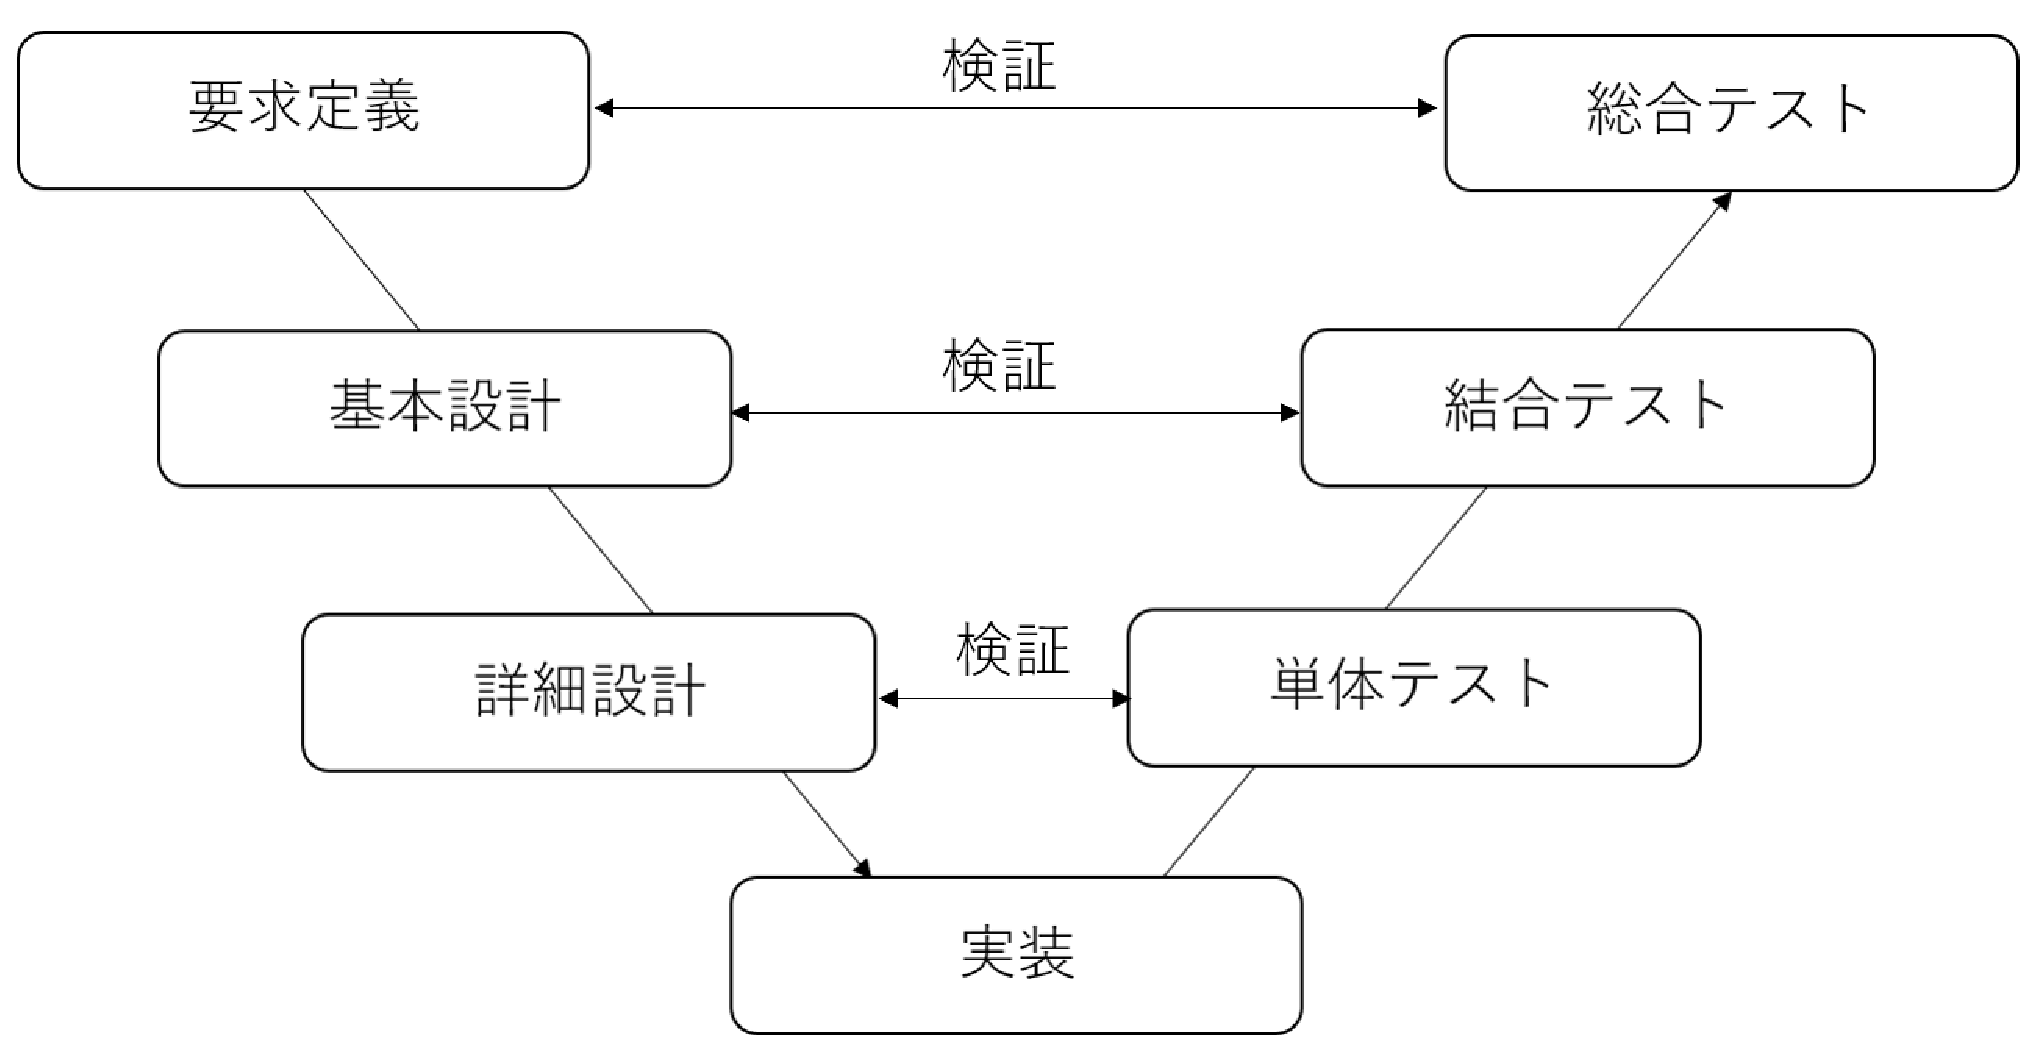
\includegraphics[width=9cm]{./vmodel2.eps}
	\caption{V字モデル}
	\label{vji}
\end{figure}


\subsection*{UML(Unifiled Modeling Language)\cite{uml}}

UMLとは統一モデリング言語(Unified Modeling Language)のことである.OMG\\(Object Management Group)と呼ばれる企業団体の標準規格として正式に承認されており,オブジェクト指向を用いている.

\subsection*{ユースケース図\cite{uml}}

ユースケース図とは,UMLで定義されている図のひとつであり,ユーザやクライアントの要求事項,システムに対して課せられている基本機能やサービス項目などの要件定義を表現するときに広く用いられる.現在考えているシステムを中心に置き,システムとその利用者(外部システムを含む)とのやりとりを表現する.利用者や外部システムをアクターとし,各アクターごとにシステムが提供する機能やサービスを識別したものをユースケースとして表現する.

\subsection*{クラス図\cite{uml}}

クラス図はUMLの基本となる図のひとつである.問題領域の構造や対象システムの静的な構成,システムの詳細設計,あるいは企業の部門の業務モデルの基本構造,問題解決の最初のとっかかりとなる概念マップの構築,といったことに広く使うことができる.クラス図を使うことで,対象システムを構成するクラス(概念や事物・事象)とそれらの間に存在する関連(意味的・物体的な繋がり)を表現できる.また,各オブジェクトがどのような属性やアクション(操作)を持っているかも合わせて記述することができる.

\subsection*{アクティビティ図\cite{uml}}

アクティビティ図とは,UMLで定義されている図のひとつであり,アプリケーションのある機能の動作の様子など,システムのワークフローを表現する.並列処理や待ち合わせ同期といった並行表現ができる.

\subsection*{シーケンス図\cite{uml}}

シーケンス図とは,UMLで定義されている相互作用図の一種であり,システムの一機能が時間経過の中でどのように動くかという動的な振る舞いを表現する.オブジェクト間のメッセージのやりとりを時系列に沿って記述するため,振る舞いを順番に追っていくのに役立つ.

\subsection*{ステートチャート図\cite{uml}}

ステートチャート図とは,UMLで定義されている図のひとつである.一つのシステムやオブジェクトのライフサイクルを状態遷移図として表現する.